\documentclass[a4paper,10pt]{article}
\usepackage[utf8]{inputenc}
\usepackage[T1]{fontenc}
\usepackage[italian]{babel}
\usepackage{graphicx}

\title{qChart - Relazione di fine progetto}
\author{Giacomo Fornari - Matricola 1029118}
\date{Giugno 2013}

\begin{document}
\maketitle

\begin{figure}[h]
    \centering
    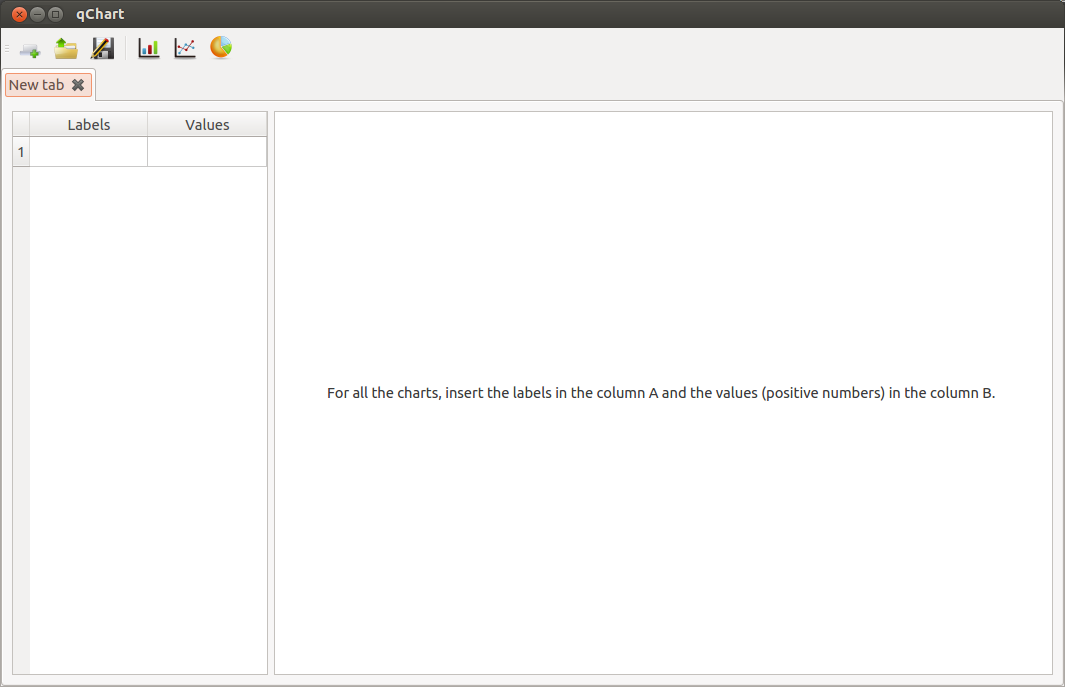
\includegraphics[scale=0.30]{gui.png}
\end{figure}

\newpage

\begin{abstract}
Il software \emph{qChart} intende dare la possibilità ad un utente di inserire e modificare dati in una tabella e, anche in momento successivo, di generare un grafico (a linee, a colonne o a torta) che rappresenti i dati inseriti.
\end{abstract}

\section{Architettura generale}
L'architettura generale è descritta dal seguente schema:

\begin{figure}[h]
    \centering
    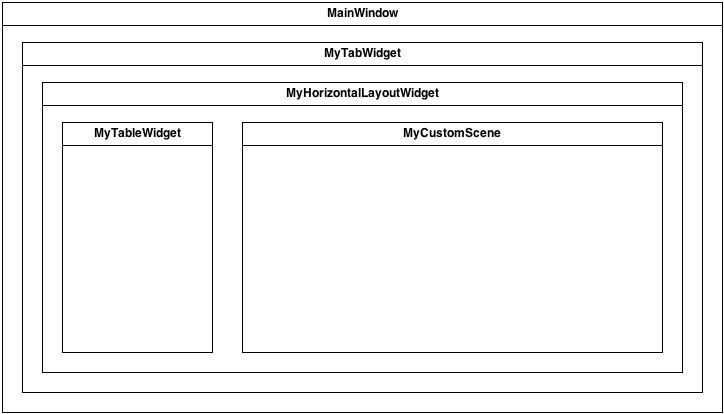
\includegraphics[scale=0.37]{architettura.png}
    \caption{Architettura generale}
\end{figure}

Tale schema viene descritto nella sezione successiva.

Nella progettazione e nello sviluppo del software si è cercato di mantenere quanto più possibile separata la parte logica dalla parte grafica. Nella progettazione si è deciso di sfruttare le classi QGraphicsScene e QGraphicsView per la visualizzazione dei grafici. Solo la prima classe è stata reimplementata per permettere l'interazione con le altre classi. In generale, le classi comunicano sfruttando il sistema di \emph{signal} e \emph{slot} reso disponibile da Qt tramite macro. Questo sistema permette una programmazione definita \emph{Event driven} poiché l'esecuzione del programma cambia al verificarsi di determinati eventi.

\section{Struttura GUI}
\paragraph{}
\emph{MainWindow} è una classe derivata direttamente da QMainWindow. Tale classe fornisce alcune funzione per l'interazione diretta con l'utente. Un attributo della classe MainWindow è un puntatore alla classe MyTabWidget, la quale viene impostata come central widget. Inoltre, MainWindow costruisce la barra dei menù e la toolbar, grazie alle quali si possono gestire gli eventi principali.

\paragraph{}
\emph{MyTabWidget} deriva direttamente da QTabWidget. Contiene come unico campo dati proprio un puntatore ad un oggetto di tipo MyHorizontalLayoutWidget. I metodi di MyTabWidget permettono la gestione delle tab e quindi di più fogli di lavoro all'interno della stessa finestra.

\paragraph{}
La classe \emph{MyHorizontalLayoutWidget} deriva direttamente da QWidget e gestisce il layout interno ad ogni tab. Infatti, come campo dati proprio ha un puntatore ad un oggetto QHBoxLayout che si occupa di organizzare tramite un layout orizzontale un oggetto MyTableWidget e un oggetto QGraphicsView. Tra gli attributi propri, presenta anche un puntatore a Chart, classe che verrà descritta nella sezione successiva. Inoltre, MyHorizontalLayoutWidget si occupa di comandare la creazione di grafici e il succcessivo passaggio degli elementi alla MyCustomScene.

\paragraph{}
La classe \emph{MyTableWidget} deriva direttamente da QTableWidget. Tale classe fornisce i metodi per la creazione e la modifica dei dati di un grafico, e l'archiviazione (e recupero) su file XML dei dati inseriti nella tabella. Queste due ultime funzioni vengono svolte dai metodi \texttt{saveXml()} e \texttt{openXml()} che, in caso di fallimento, sollevano delle eccezioni. La classe fornisce la funzione di aggiungere righe alla fine della tabella e di cancellare la riga corrente. Per fare ciò, è stato eseguito l'overriding del metodo virtuale \emph{keyPressEvent} ereditato da QAbstractItemView, in modo tale da inserire righe con il tasto Enter e cancellarne con il tasto Delete. Il numero di colonne che costituiscono la tabella è fisso. Nella prima colonna si può inserire qualsiasi tipo di valore, mentre nella seconda sono accettati solo valori numerici positivi. Ogni valore inserito nelle celle della seconda colonna vieni controllato da un oggetto QValidator; se non soddisfa i requisiti, viene inserita una stringa vuota.

MyTableWidget fornisce i metodi \texttt{QVector<QString> getColumnString(int index=0)} e \texttt{QVector<double> getColumnDouble(int index=1)} per ritornare i dati della colonna \texttt{index} con tipo definito dal prototipo. Se in una cella non è ancora stato istanziato un item o quando il testo è una stringa vuota, il secondo metodo restituisce zero come valore corrispondente a quella cella.

\paragraph{}
\emph{MyCustomScene} deriva direttamente da QGraphicsScene. Tale classe rappresenta sulla scena gli oggetti di tipo QGraphicsItem e li mette a disposizione della classe QGraphicsView che li mostra all'utente. Se il numero di elementi da visualizzare è elevato e lo spazio risulta insufficiente, viene sfruttata una scrollbar generata automaticamente data la derivazione di QGraphicsView da QAbstractScrollArea. Gli oggetti QGraphicsItem le vengono passati dalle classi chart con tutti i parametri già definiti, in tal modo il compito di MyCustomScene si riduce ad aggiungere gli elementi alla scena.

\newpage
\section{Gerarchia \texttt{Chart}}
La struttura della gerarchia \emph{Chart} implementata è rappresentata dal seguente schema:

\begin{figure}[h]
    \centering
    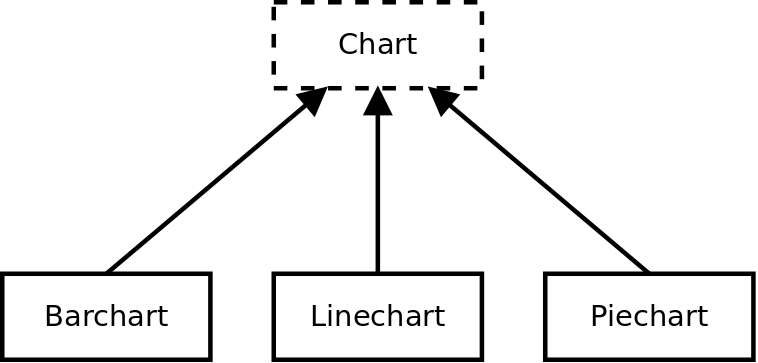
\includegraphics[scale=0.3]{chart.png}
    \caption{Gerarchia Chart}
\end{figure}

\subsection{Chart}
\emph{Chart} è la classe base astratta comune a tutte le classi che intendono creare oggetti per un chart. Fornisce dei metodi virtuali puri quali:
\begin{itemize}
	\item \emph{makeItems()} per la creazione degli oggetti di tipo QGraphicsItem
	\item \emph{returnItems()} necessaria per ritornare una QList<QGraphicsItem *>, ovvero una lista gli oggetti creati 
	\item \emph{normalize()} per normalizzare i dati utili alla generazione degli oggetti grafici.
\end{itemize}

\subsection{Barchart}
\emph{Barchart} è una classe concreta che deriva da Chart e reimplementa i metodi virtuali puri.

Il metodo makeItems() crea gli assi, le colonne e le etichette sulla base dei dati normalizzati da normalize(). I dati vengono normalizzati in base ad un parametro fissato a 480. Dunque, i valori massimi del vettore di dati saranno uguali a 480 dopo la normalizzazione. Le colonne sono create sulla base dei dati normalizzati, dunque quell relative ai valori massimi corrisponderanno ad un altezza di 480 pixel sulla scena. Le etichette vengono passate come figli delle colonne e posizionate al di sotto di esse.

Gli oggetti generati vengono appesi alla lista che verrà passata successivamente alla scena.

\subsection{Linechart}
\emph{Linechart} è una classe concreta che deriva da Chart e reimplementa i metodi virtuali puri.

Il metodo makeItems() crea gli assi, le linee principali e le etichette sulla base dei dati normalizzati da normalize(). Anche in questo caso i dati vengono normalizzati a 480. I punti rappresentanti ai valori massimi saranno a 480 pixel di distanza dall'asse orizzontale. Le etichette vengono posizionate in corrispondenza dei valori a cui sono associati e tutte equispaziate lungo l'asse orizzontale.

Gli oggetti generati vengono appesi alla lista che verrà passata successivamente alla scena.

\subsection{Piechart}
\emph{Piechart} è una classe concreta che deriva da Chart e reimplementa i metodi virtuali puri.

Il metodo makeItems() crea le fette della torta e i tooltips associati ad esse. Il metodo normalize() normalizza i dati in modo che la loro somma sia uguale a 5780, valore corrispondente all'angolo giro in Qt. Gli spicchi del cerchio sono oggetti della classe \emph{MyGraphicsEllipseItem}, una derivazione della classe QGraphicsEllipdeItem. Questa derivazione è stata necessaria per eseguire l'overriding dei metodi virtuali \emph{hoverEnterEvent} e \emph{hoverLeaveEvent} per implementare gli eventi attivati dal passaggio del cursore del mouse sugli oggetti. Infatti, chiamando il metodo hoverEnterEvent il colore dell'oggetto perde di opacità, mentre chiamando hoverLeaveEvent torna allo stato precendente. Le etichette vengono aggiunte come tooltip all'oggetto corrispondente.

Se al momento della creazione del grafico non sono presenti valori diversi da zero nella seconda colonna, non verrà creato creato l'oggetto Piechart.

Gli oggetti generati vengono appesi alla lista che verrà passata successivamente alla scena.

\appendix
\section{Specifiche tecniche di sviluppo}
Il software è stato sviluppato sulle seguenti specifiche:
\begin{itemize}
	\item[]Sistema operativo: Ubuntu 12.04 LTS
	\item[]Compilatore: GCC 4.6.3
	\item[]Librerie: Qt 4.8.0
\end{itemize}
Per compilare il progetto utilizzare i comandi \texttt{qmake} e \texttt{make}.

\end{document}